\documentclass{article}

\usepackage{graphicx}
\usepackage{float}
\usepackage{amsmath}
\usepackage{booktabs}
\usepackage{fullpage}
\usepackage{bm}
\usepackage{amssymb}

\DeclareMathOperator*{\argmax}{arg\,max}

\makeatletter
\renewcommand*\env@matrix[1][*\c@MaxMatrixCols c]{%
  \hskip -\arraycolsep
  \let\@ifnextchar\new@ifnextchar
  \array{#1}}
\makeatother

% Default fixed font does not support bold face
\DeclareFixedFont{\ttb}{T1}{txtt}{bx}{n}{9} % for bold
\DeclareFixedFont{\ttm}{T1}{txtt}{m}{n}{9}  % for normal

% Custom colors
\usepackage{color}
\definecolor{deepblue}{rgb}{0,0,0.5}
\definecolor{deepred}{rgb}{0.6,0,0}
\definecolor{deepgreen}{rgb}{0,0.5,0}

\usepackage{listings}

% Python style for highlighting
\newcommand\pythonstyle{\lstset{
language=Python,
basicstyle=\ttm,
otherkeywords={self},             % Add keywords here
keywordstyle=\ttb\color{deepblue},
emph={MyClass,__init__},          % Custom highlighting
emphstyle=\ttb\color{deepred},    % Custom highlighting style
stringstyle=\color{deepgreen},
frame=tb,                         % Any extra options here
showstringspaces=false            % 
}}


% Python environment
\lstnewenvironment{python}[1][]
{
\pythonstyle
\lstset{#1}
}
{}

\title{Statistical Machine Learning: Assignment 2}
\date{\today}
\author{Joris van Vugt, s4279859}

\begin{document}
\maketitle
\section*{Exercise 1 -- Sequential learning}
\subsection*{Part 1 -- Obtaining the prior}
\begin{enumerate}
\item 
First we compute the precision matrix using \texttt{numpy.linalg.inv}:
$$
\tilde{\bm{\Lambda}} = \tilde{\bm{\Sigma}}^{-1} = 
\begin{pmatrix}[c c | c c]
60 & 50 & -48 & 38 \\
50 & 50 & -50 & 40 \\ \hline
-48 & -50 & 52.4 & -41.4 \\
38 & 40 & -41.4 & 33.4
\end{pmatrix} = 
\begin{pmatrix}[c | c]
\tilde{\bm{\Lambda}}_{aa} & \tilde{\bm{\Lambda}}_{ab} \\
\hline
\tilde{\bm{\Lambda}}_{ba} & \tilde{\bm{\Lambda}}_{bb} \\
\end{pmatrix}
$$
Now, using equations 2.73 and 2.75 from Bishop, we can compute the conditional covariance:
$$
\bm{\Sigma}_p = \tilde{\bm{\Lambda}}_{aa}^{-1} = 
\begin{pmatrix}
0.1 & -0.1 \\
-0.1 & 0.12
\end{pmatrix}
$$
and the conditional mean:
\begin{align*}
\bm{\mu}_p &= \bm{\mu}_a - \tilde{\bm{\Lambda}}_{aa}^{-1} \tilde{\bm{\Lambda}}_{ab}(\bm{x}_b - \bm{\mu}_b) \\
&= \begin{pmatrix}1 \\ 0 \end{pmatrix} - 
\begin{pmatrix}
0.1 & -0.1 \\
-0.1 & 0.12
\end{pmatrix}
\begin{pmatrix}
-48 & 38 \\
-50 & 40
\end{pmatrix}
\Bigg[\begin{pmatrix}0 \\ 0\end{pmatrix} - \begin{pmatrix}1 \\ 2\end{pmatrix}\Bigg] \\
&= \begin{pmatrix}1 \\ 0 \end{pmatrix} - 
\begin{pmatrix}
0.1 & -0.1 \\
-0.1 & 0.12
\end{pmatrix}
\begin{pmatrix}
-48 & 38 \\
-50 & 40
\end{pmatrix}
\begin{pmatrix}-1 \\ -2\end{pmatrix} \\
&= \begin{pmatrix}1 \\ 0 \end{pmatrix} - 
\begin{pmatrix}
0.2 & -0.2 \\
-1.2 & 1
\end{pmatrix}
\begin{pmatrix}-1 \\ -2\end{pmatrix} \\
&= \begin{pmatrix}1 \\ 0 \end{pmatrix} - 
\begin{pmatrix}0.2 \\ -0.8 \end{pmatrix} \\
&= \begin{pmatrix}0.8 \\ 0.8 \end{pmatrix}
\end{align*}
\item 
\begin{python}
def generate_pair():
    return np.random.multivariate_normal([0.8, 0.8], 
    					 [[0.1, -0.1],
    	 				  [-0.1, 0.12]])
\end{python}
$$
\bm{\mu}_t=\begin{pmatrix}0.28 \\ 1.18 \end{pmatrix}
$$
\item
To calculate the probability density of our multivariate Gaussian random variable, we use \\ \texttt{scipy.stats.multivariate\_normal} and its \texttt{pdf} method.
\begin{python}
x, y = np.mgrid[-0.25:2.25:.01, -1:2:.01]
pos = np.empty(x.shape + (2,))
pos[:, :, 0] = x
pos[:, :, 1] = y
mu_p = [0.8, 0.8]
cov_p = [[0.1, -0.1], [-0.1, 0.12]]
z = multivariate_normal(mu_p, cov_p).pdf(pos)

fig = plt.figure()
ax = fig.gca(projection='3d')
ax.plot_surface(x, y, z, cmap=plt.cm.viridis)
# More plot formatting code
\end{python}
\begin{figure}[H]
\centering
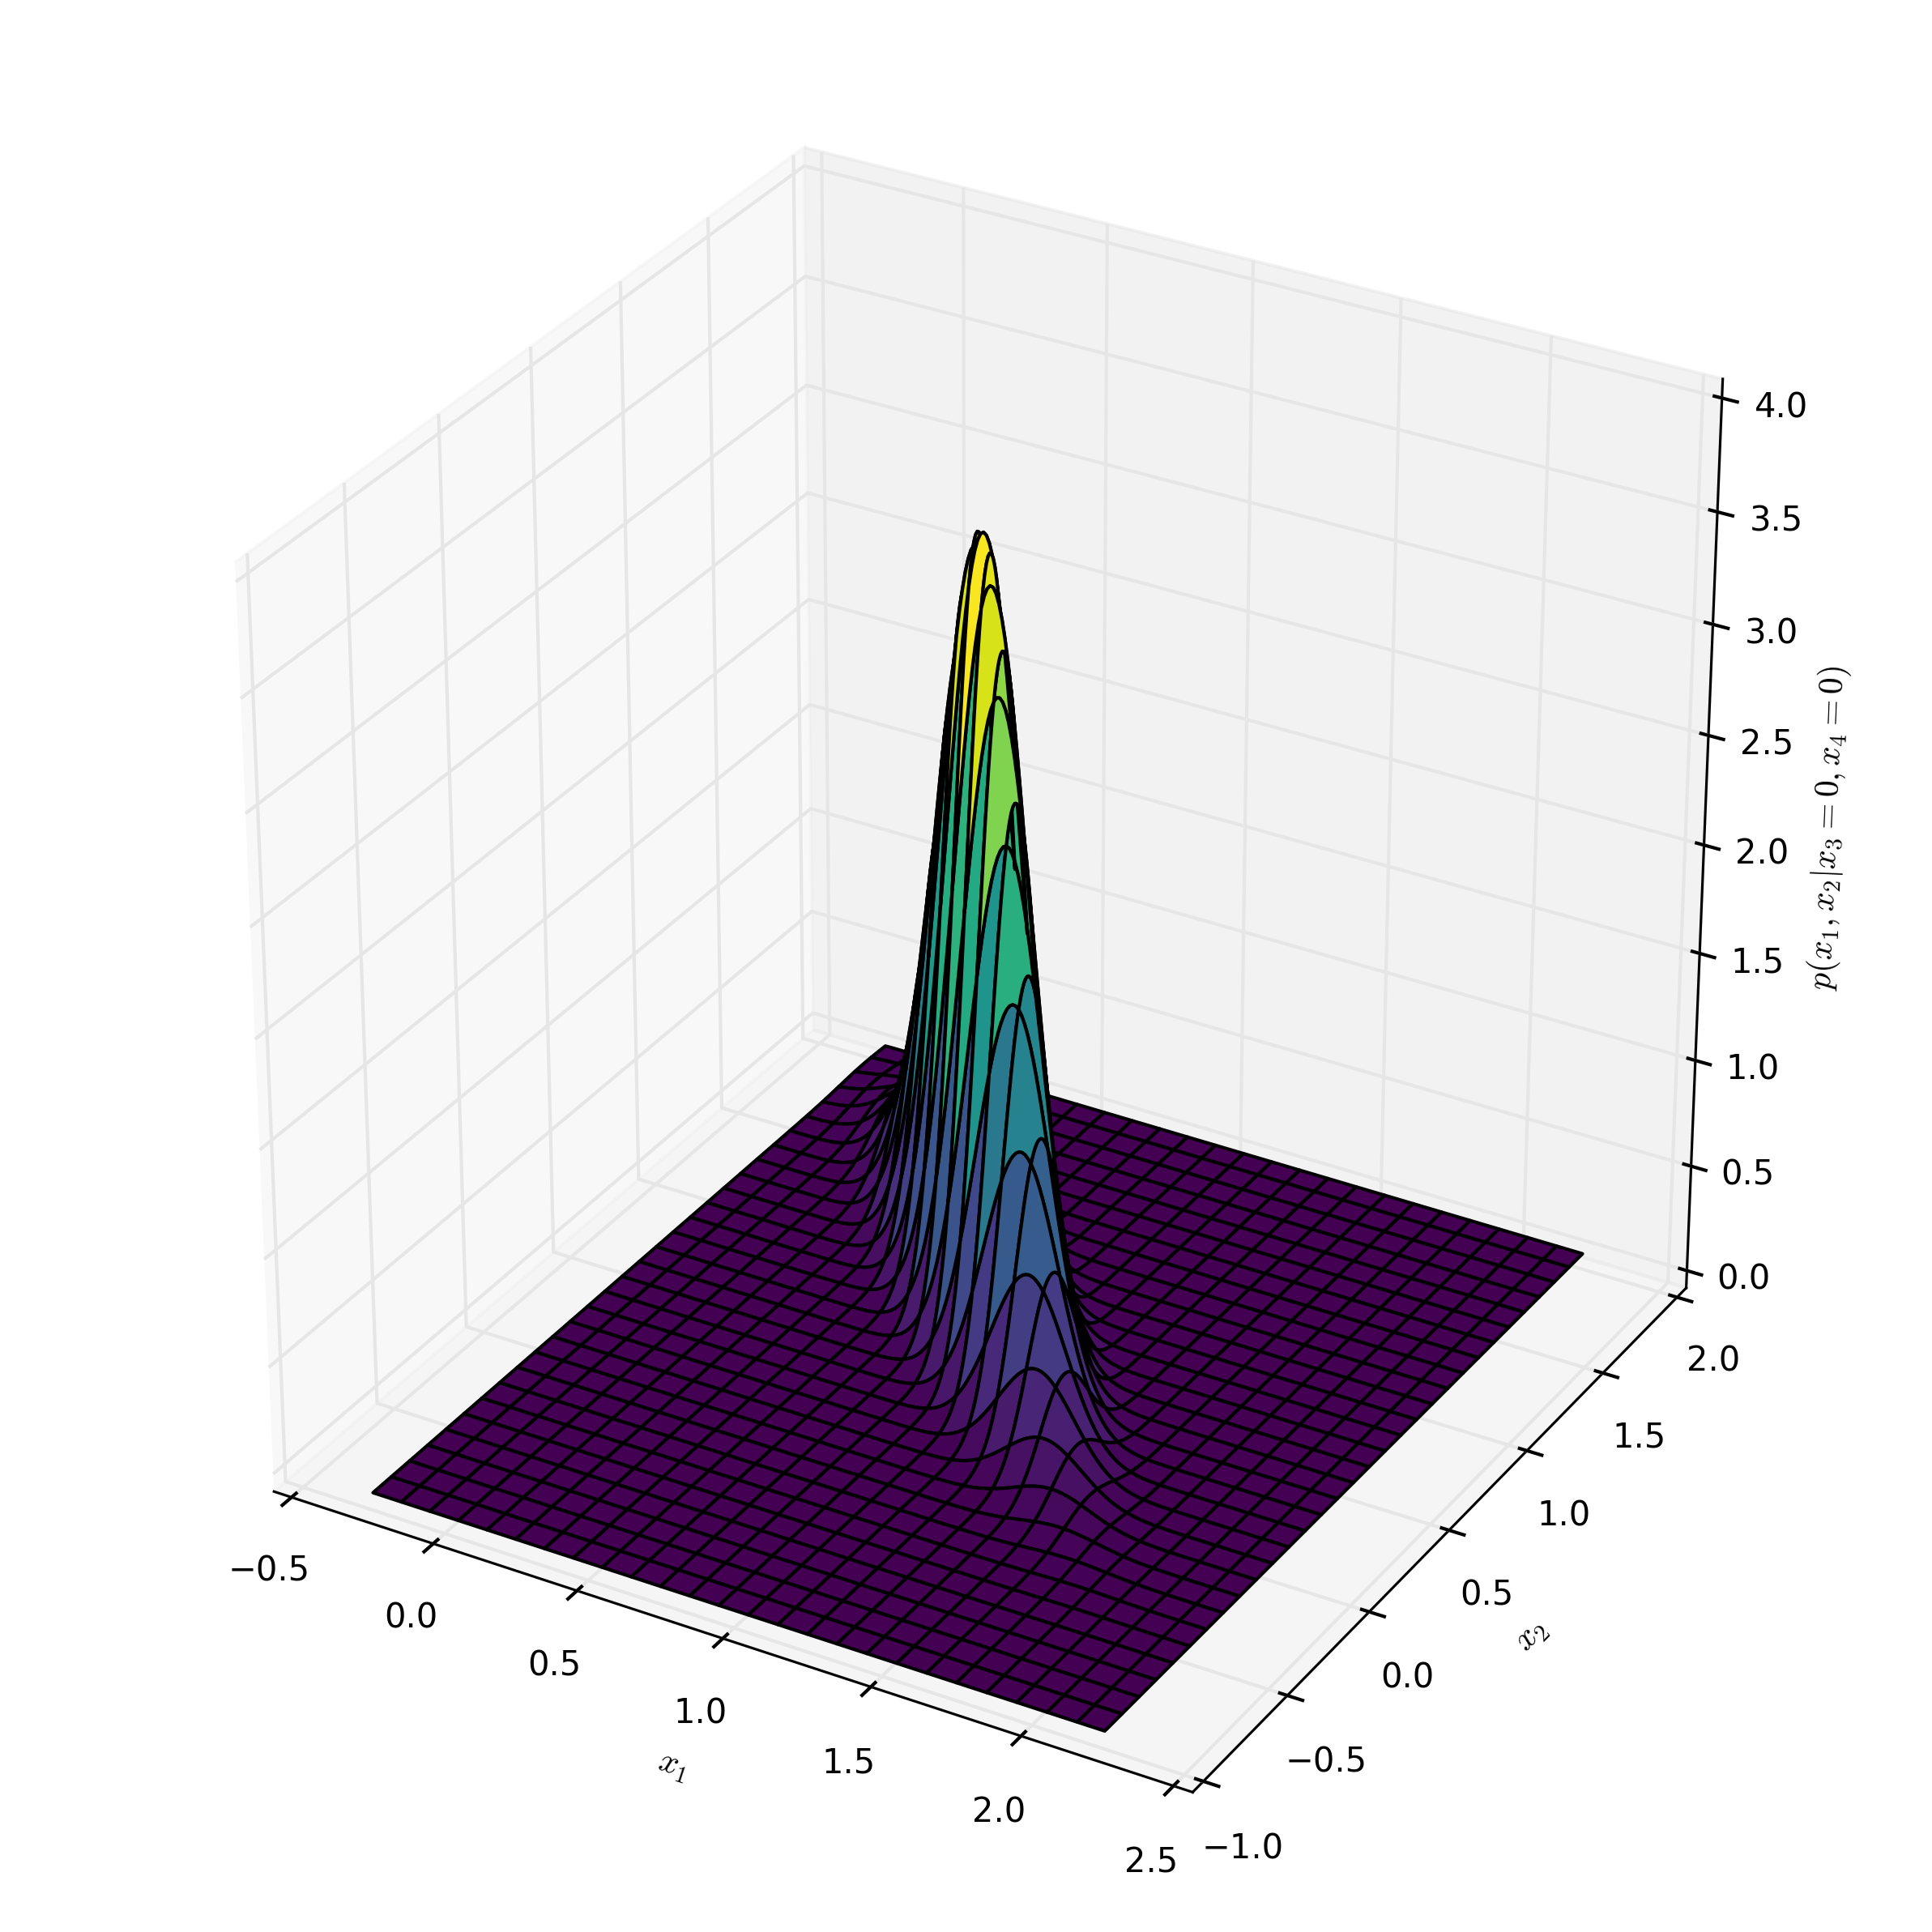
\includegraphics[width=.6\textwidth]{images/cond_mvg.png}
\caption{Probability density plot of the multivariate Gaussian (Ex 1.1.3)}
\label{fig:cond_mvg}
\end{figure}
\end{enumerate}
\pagebreak
\subsection*{Part 2 -- Generating the data}
\begin{enumerate}
\item 
\begin{python}
N = 1000
data = np.random.multivariate_normal([0.28, 1.18], 
				     [[2.0, 0.8], 
				      [0.8, 4.0]], 
				     N)
np.savetxt('data.txt', data)
\end{python}
\item The maximum likelihood estimate of the mean is simply the mean of the observed data:
$$
\bm{\mu}_\text{ML} = \frac{1}{N}\sum_{n=1}^N\bm{x}_n = \begin{pmatrix}0.25 \\ 1.21 \end{pmatrix}
$$
Computing the maximum likelihood estimate of the covariance is slightly more involved:
$$
\bm{\Sigma}_\text{ML} = \frac{1}{N}\sum_{n=1}^N(\bm{x}_n - \bm{\mu}_\text{ML})(\bm{x}_n - \bm{\mu}_\text{ML})^T = 
\begin{pmatrix}
2.023 & 0.828 \\
0.828 & 3.626
\end{pmatrix}
$$
To compute the unbiased maximum likelihood covariance estimate, we normalize by $N - 1$ instead of $N$:
$$
\bm{\Sigma}_\text{ML} = \frac{1}{N - 1}\sum_{n=1}^N(\bm{x}_n - \bm{\mu}_\text{ML})(\bm{x}_n - \bm{\mu}_\text{ML})^T = 
\begin{pmatrix}
2.025 & 0.829 \\
0.829 & 3.629
\end{pmatrix}
$$
These results were obtained with the following code:
\begin{python}
mu_ml = data.mean(axis=0)
x = data - mu_ml
cov_ml = np.dot(x.T, x) / N
cov_ml_unbiased = np.dot(x.T, x) / (N - 1)
\end{python}
Note that the left factor is transposed instead of the right factor in the covariance estimates. This is because our points are row vectors instead of column vectors (i.e., \texttt{data} has shape $N \times 2$).

\par We can compare our estimates to the true statistics:
$$
\bm{\mu}_t = \begin{pmatrix} 0.28 \\ 1.18\end{pmatrix} \hspace{2em} \bm{\Sigma}_t = \begin{pmatrix} 2.0 & 0.8 \\ 0.8 & 4.0 \end{pmatrix}
$$
Our estimates are pretty close to their true values. The unbiased estimate of the covariance is not much closer than the biased estimate. Because N is relatively high, the slight change in normalization does not have much effect.
\end{enumerate}
\pagebreak
\subsection*{Part 3 -- Sequential learning algorithms}
\begin{enumerate}
\item Using equation 2.126 from Bishop
$$
\bm{\mu}_\text{ML}^{(N)} = \bm{\mu}_\text{ML}^{(N-1)} + \frac{1}{N}(\bm{x}_N - \bm{\mu}_\text{ML}^{(N-1)})
$$
we can come up with a Python procedure for sequential learning:
\begin{python}
def seq_ml(data):
    mus = [np.array([[0], [0]])]
    for i in range(N):
        x_n = data[i].reshape(2, 1)
        mu_n = mus[-1] + (x_n-mus[-1]) / (i + 1)
        mus.append(mu_n)
    return mus
\end{python}
The starting value $\bm{\mu}_\text{ML}^{(0)}$ does not matter, but is arbitrarily set to $\begin{pmatrix}0 \\ 0\end{pmatrix} $. We divide by $i + 1$ instead of just $i$, because Python uses 0-based indexing.
\item
We can use equation 2.113 from Bishop\footnote{With mappings 
$\bm{x} = \bm{\mu}$, 
$\bm{\mu}=\bm{\mu}_{(n-1)}$ and 
$\bm{\Lambda}^{-1} = \bm{\Sigma}_{(n-1)} $}
$$
P(\bm{\mu} | D_{n-1}) = \mathcal{N}(\bm{\mu} | \bm{\mu}_{(n-1)}, \bm{\Sigma}_{(n-1)})
$$
and equation 2.114 from Bishop\footnote{With mappings
$\bm{y} = \bm{x}_n$,
$\bm{A} = \bm{I}$,
$\bm{x} = \bm{\mu}$,
$\bm{b} = 0$ and
$\bm{L}^{-1} = \bm{\Sigma}_t$}
$$
P(\bm{x}_n | \bm{\mu}, D_{n-1}) = \mathcal{N}(\bm{x}_n | \bm{\mu}, \bm{\Sigma}_t).
$$
Now we can apply equation 2.116 from Bishop to find out the posterior
$$
P(\bm{\mu} | \bm{x}_n D_{n-1}) = \mathcal{N}(\bm{\mu} | \bm{\Sigma}\{\bm{\Sigma}_t^{-1}\bm{x}_n + \bm{\Sigma}_{(n-1)}^{-1}\bm{\mu}_{(n-1)}\}, \bm{\Sigma}).
$$
Equation 2.117 gives us
$$
\bm{\Sigma} = (\bm{\Sigma}_{(n-1)}^{-1} + \bm{\Sigma}_t^{-1})^{-1}.
$$
The sequential learning rules for the mean and the covariance are thus
\begin{align*}
\bm{\mu}_{(n)} &=  \bm{\Sigma}_{(n)}\{\bm{\Sigma}_t^{-1}\bm{x}_n + \bm{\Sigma}_{(n-1)}^{-1}\bm{\mu}_{(n-1)}\} \\
\bm{\Sigma}_{(n)} &= (\bm{\Sigma}_{(n-1)}^{-1} + \bm{\Sigma}_t^{-1})^{-1}
\end{align*}
\item 
\begin{python}
def seq_map(data, mu_p, cov_p, cov_t):
    mus, covs = [mu_p], [cov_p]
    for x in data:
        x_n = x.reshape(2, 1)
        cov_n = np.linalg.inv(np.linalg.inv(covs[-1]) + np.linalg.inv(cov_t))
        mu_n = cov_n.dot(np.linalg.inv(cov_t).dot(x_n) + np.linalg.inv(covs[-1]).dot(mus[-1]))
        mus.append(mu_n)
        covs.append(cov_n)
        
    return mus, covs
\end{python}
\item
\begin{figure}[H]
\centering
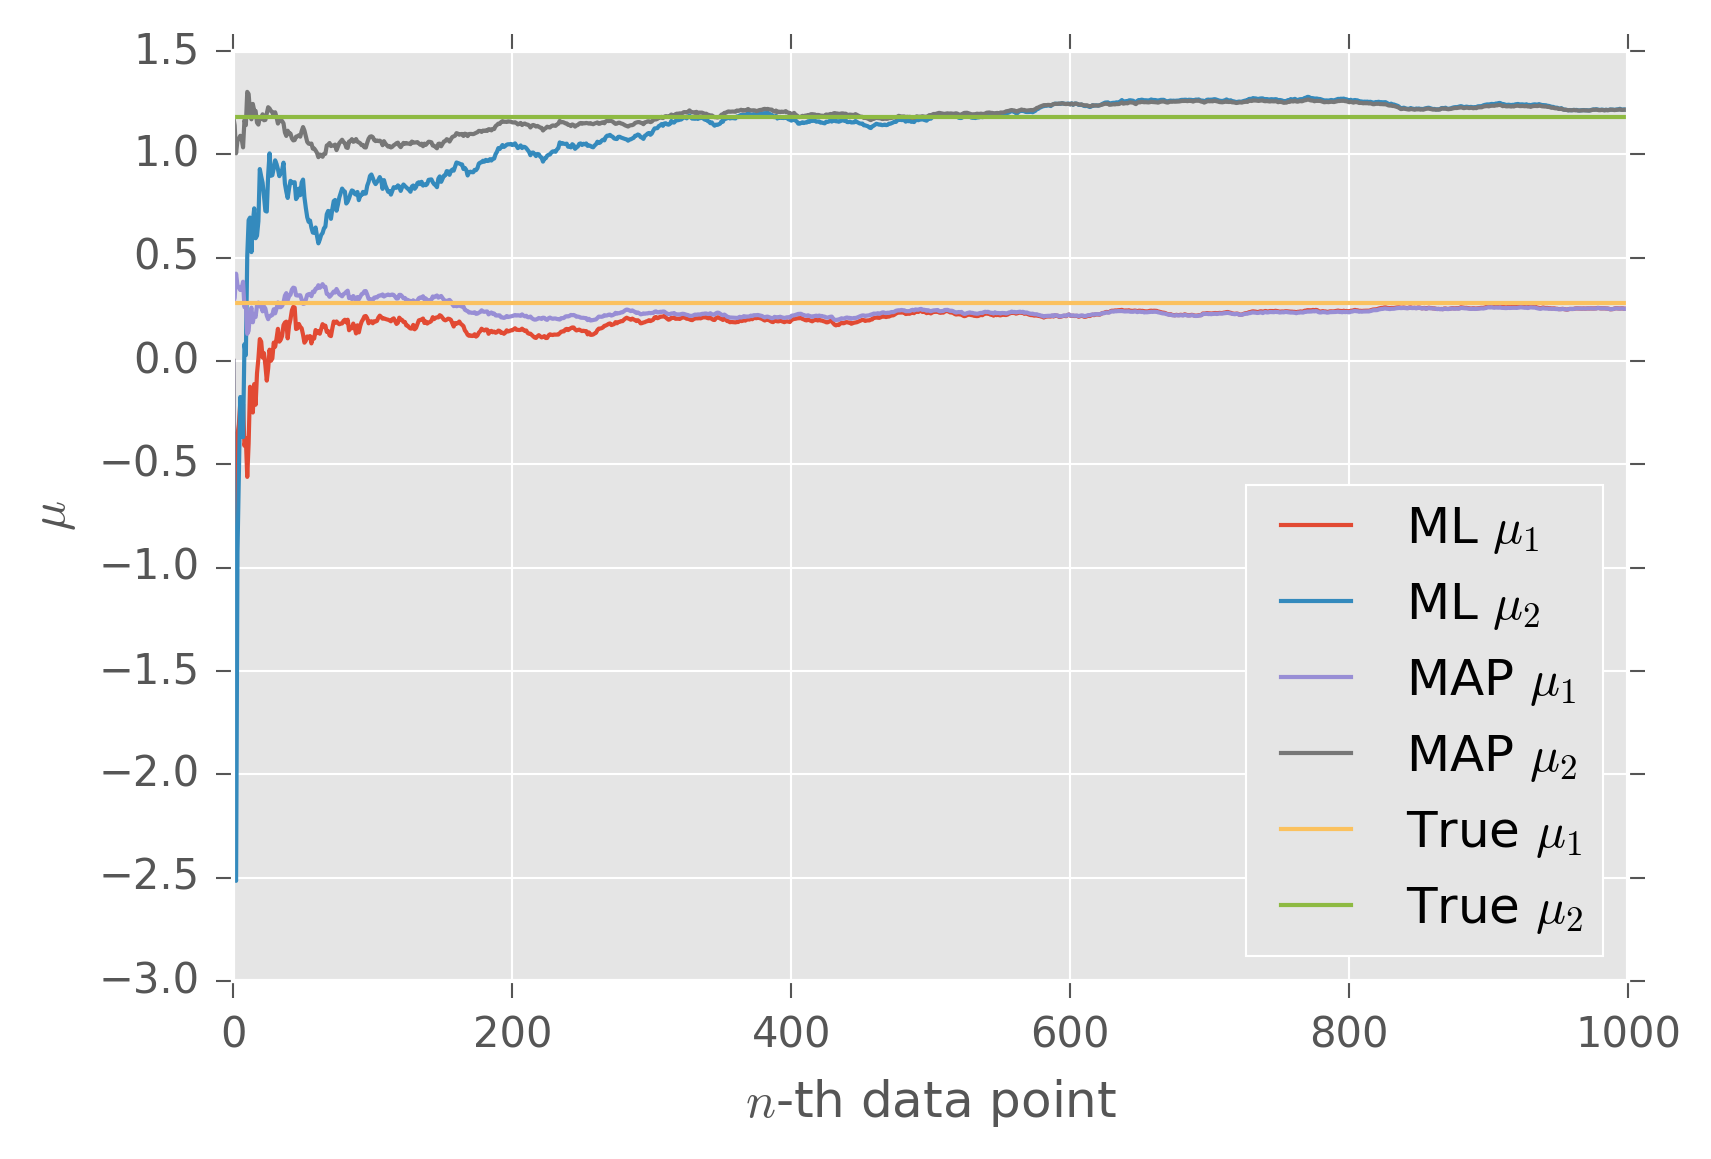
\includegraphics[width=0.8\textwidth]{images/seq_learning.png}
\caption{The ML and MAP estimates for both components of $\mu$ as a function of the number of data points observed. (Ex 1.3.4)}
\end{figure}
Both the ML and MAP estimates converge to the true values quite quickly. Because a reasonable prior is chosen, the MAP converges a bit faster. After enough data points, the effect of the prior becomes negligable and the ML and MAP estimates are roughly equal.
\end{enumerate}

\section*{Exercise 2 -- The faulty lighthouse}
\subsection*{Part 1 -- Constructing the model}
\begin{enumerate}
\item 
The photo-detectors are located on the coast and thus only half of the angles can be observed, namely those towards the coast. A full circle corresponds to $2\pi$. We can only observe half a circle, so $p(\theta_k|\alpha, \beta) = \frac{1}{\pi}$ indicates a uniform distribution over all possible angles. We can show that this distribution integrates to 1 and is thus a valid probability distribution
\begin{align*}
\int_{-\frac{\pi}{2}}^{\frac{\pi}{2}}\frac{1}{\pi} &= \frac{x}{\pi}\Big|_{-\frac{\pi}{2}}^{\frac{\pi}{2}} \\
&= \frac{\frac{\pi}{2} + \frac{\pi}{2}}{\pi} = 1.
\end{align*}
\item 
Rewriting equation 7 gives
$$
\theta_k = \tan^{-1}(\frac{x_k - \alpha}{\beta}).
$$
We also need the Jacobian
\begin{align*}
\big|\frac{\text{d}\theta}{\text{d}x}\big| &= \frac{1}{1+(\frac{x_k - \alpha}{\beta})^2} \times \frac{\beta}{\beta^2} \\
&= \frac{\beta}{\beta^2+\beta^2(\frac{x_k - \alpha}{\beta})^2} \\
&= \frac{\beta}{\beta^2+(x_k - \alpha)^2} \\
\end{align*}
multiplying these gives the expected distribution over $x_k$
\begin{align*}
p(x_k | \alpha, \beta) &= p(\theta_k)\bigg|\frac{\text{d}\theta}{\text{d}x}\bigg| \\
&= \frac{1}{\pi} \times \frac{\beta}{\beta^2+(x_k - \alpha)^2} \\
&= \frac{\beta}{\pi[\beta^2+(x_k - \alpha)^2]}
\end{align*}
\begin{figure}[H]
\centering
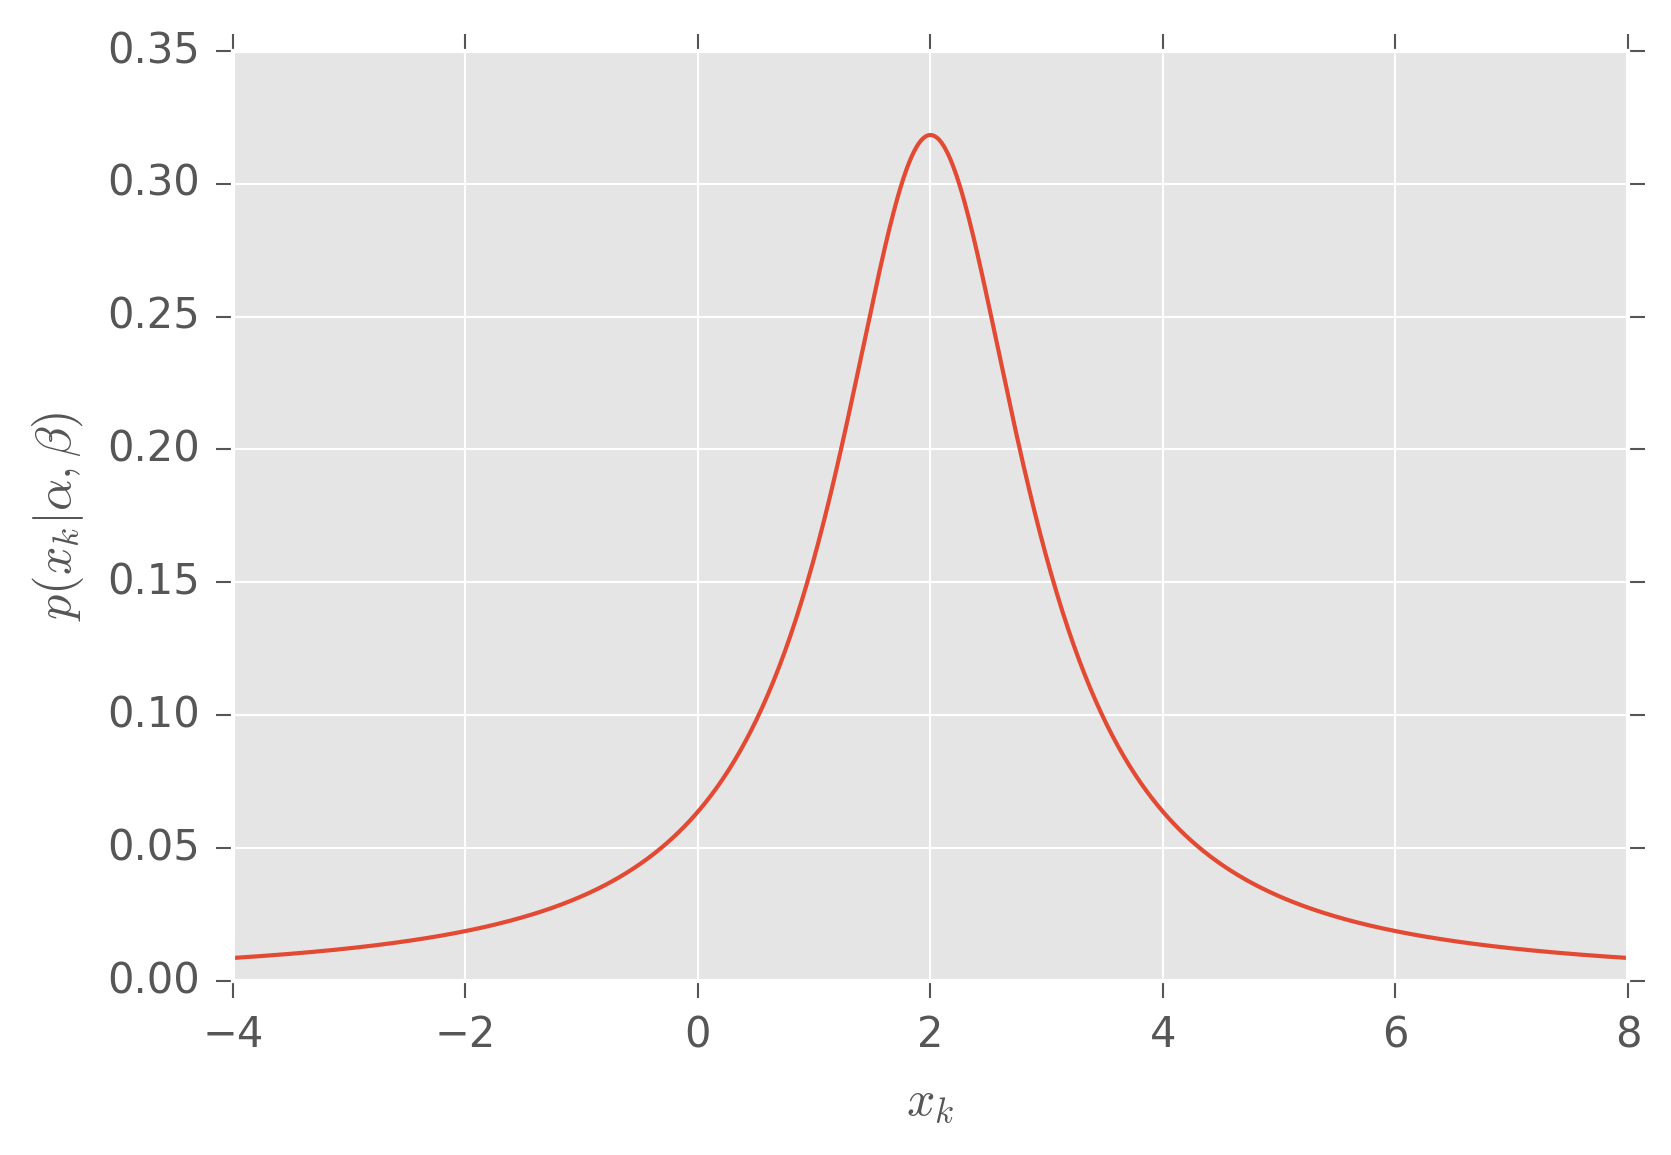
\includegraphics[width=.6\textwidth]{images/prob_xk.png}
\caption{The probability distribution $p(x_k | \alpha=2, \beta=1)$ (Ex 2.2.2)}
\end{figure}
\begin{python}
def p_xk(x, alpha, beta):
    return beta / (np.pi * (beta**2 + (x-alpha)**2))

x = np.linspace(-4, 8, num=1000)
probs = p_xk(x, 2, 1)
plt.plot(x, probs)
\end{python}
\item 
According to $p(\alpha | \mathcal{D}, \beta) \propto p(\mathcal{D} | \alpha, \beta)p(\alpha|\beta)$, we just need to calculcate  $p(\mathcal{D} | \alpha, \beta)$, since $p(\alpha|\beta)$ does not depend on the data. $p(\mathcal{D} | \alpha, \beta)$ is simply the product of the probability of each data point. We can now calculate log of the posterior density 

\begin{align*}
L &= \ln(p(\alpha | \mathcal{D}, \beta)) \\
&= \ln(\prod_{k=1}^N \frac{\beta}{\pi[\beta^2+(x_k - \alpha)^2]}) \\
&= \sum_{k=1}^N \ln\bigg(\frac{\beta}{\pi}\times\frac{1}{\beta^2+(x_k - \alpha)^2}\bigg) \\
&= N\ln\frac{\beta}{\pi} - \sum_{k=1}^N \ln[\beta^2+(x_k - \alpha)^2] \\
&= \textit{constant } - \sum_{k=1}^N \ln[\beta^2+(x_k - \alpha)^2]
\end{align*}
and an expression for maximizing this density
\begin{align*}
\hat{\alpha} &= \argmax_a \sum_{k=1}^N \ln[\beta^2+(x_k - \alpha)^2]\\
\end{align*}
\item 
\begin{figure}[H]
\centering
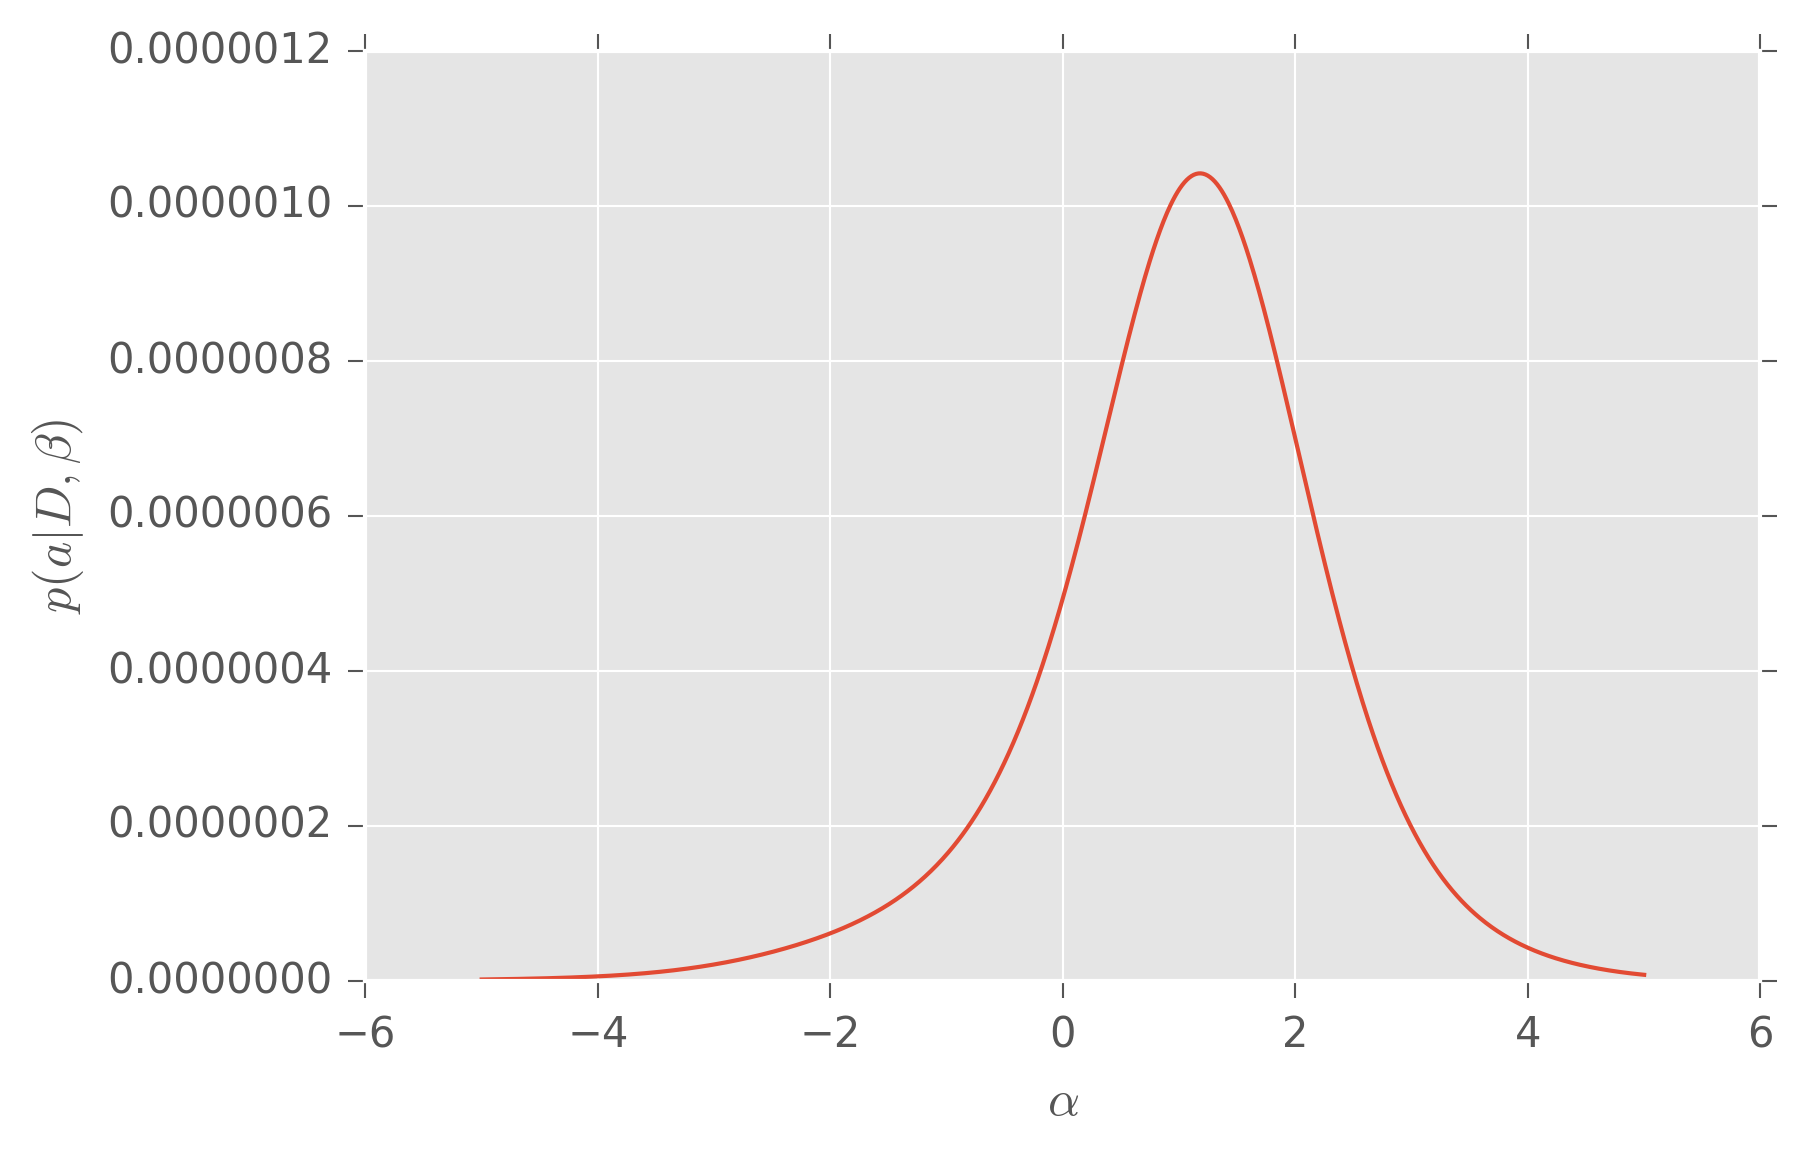
\includegraphics[width=.6\textwidth]{images/prob_a.png}
\caption{Probability density of $\alpha$ (Ex 2.1.4)}
\end{figure}
\begin{python}
def p_a(x, alpha, beta):
    return np.product(beta / (np.pi * beta**2 + (x-alpha)**2))

D = np.array([4.8, -2.7, 2.2, 1.1, 0.8, -7.3])
alphas = np.linspace(-5, 5, num=1000)
beta = 1
likelihoods = [p_a(D, alpha, beta) for alpha in alphas]
plt.plot(alphas, likelihoods)
\end{python}
The mean of the data is -0.183, but the maximum likelood is $\hat{\alpha}\approx 1.18$. The discrepancy might be the result of the small size of the data set.
\end{enumerate}
\subsection*{Part 2 -- Generate the lighthouse data}
\begin{enumerate}
\item 
\begin{python}
alpha_t = np.random.uniform(0, 10)
beta_t = np.random.uniform(1, 2)
\end{python}
We have $\alpha_t = 6.03$ and $\beta_t=1.76$.
\item 
Given an angle, we need to calculate the position it will be detected at
\begin{align*}
\beta \tan(\theta) &= x - \alpha \\
x &=  \beta \tan(\theta) + \alpha
\end{align*}
\begin{python}
def location(angle, alpha, beta):
    return beta * np.tan(angle) + alpha

N = 200
angles = np.random.uniform(-np.pi/2, np.pi/2, N)
locations = [location(angle, alpha_t, beta_t) for angle in angles]
\end{python}
\item 
\begin{figure}[H]
\centering
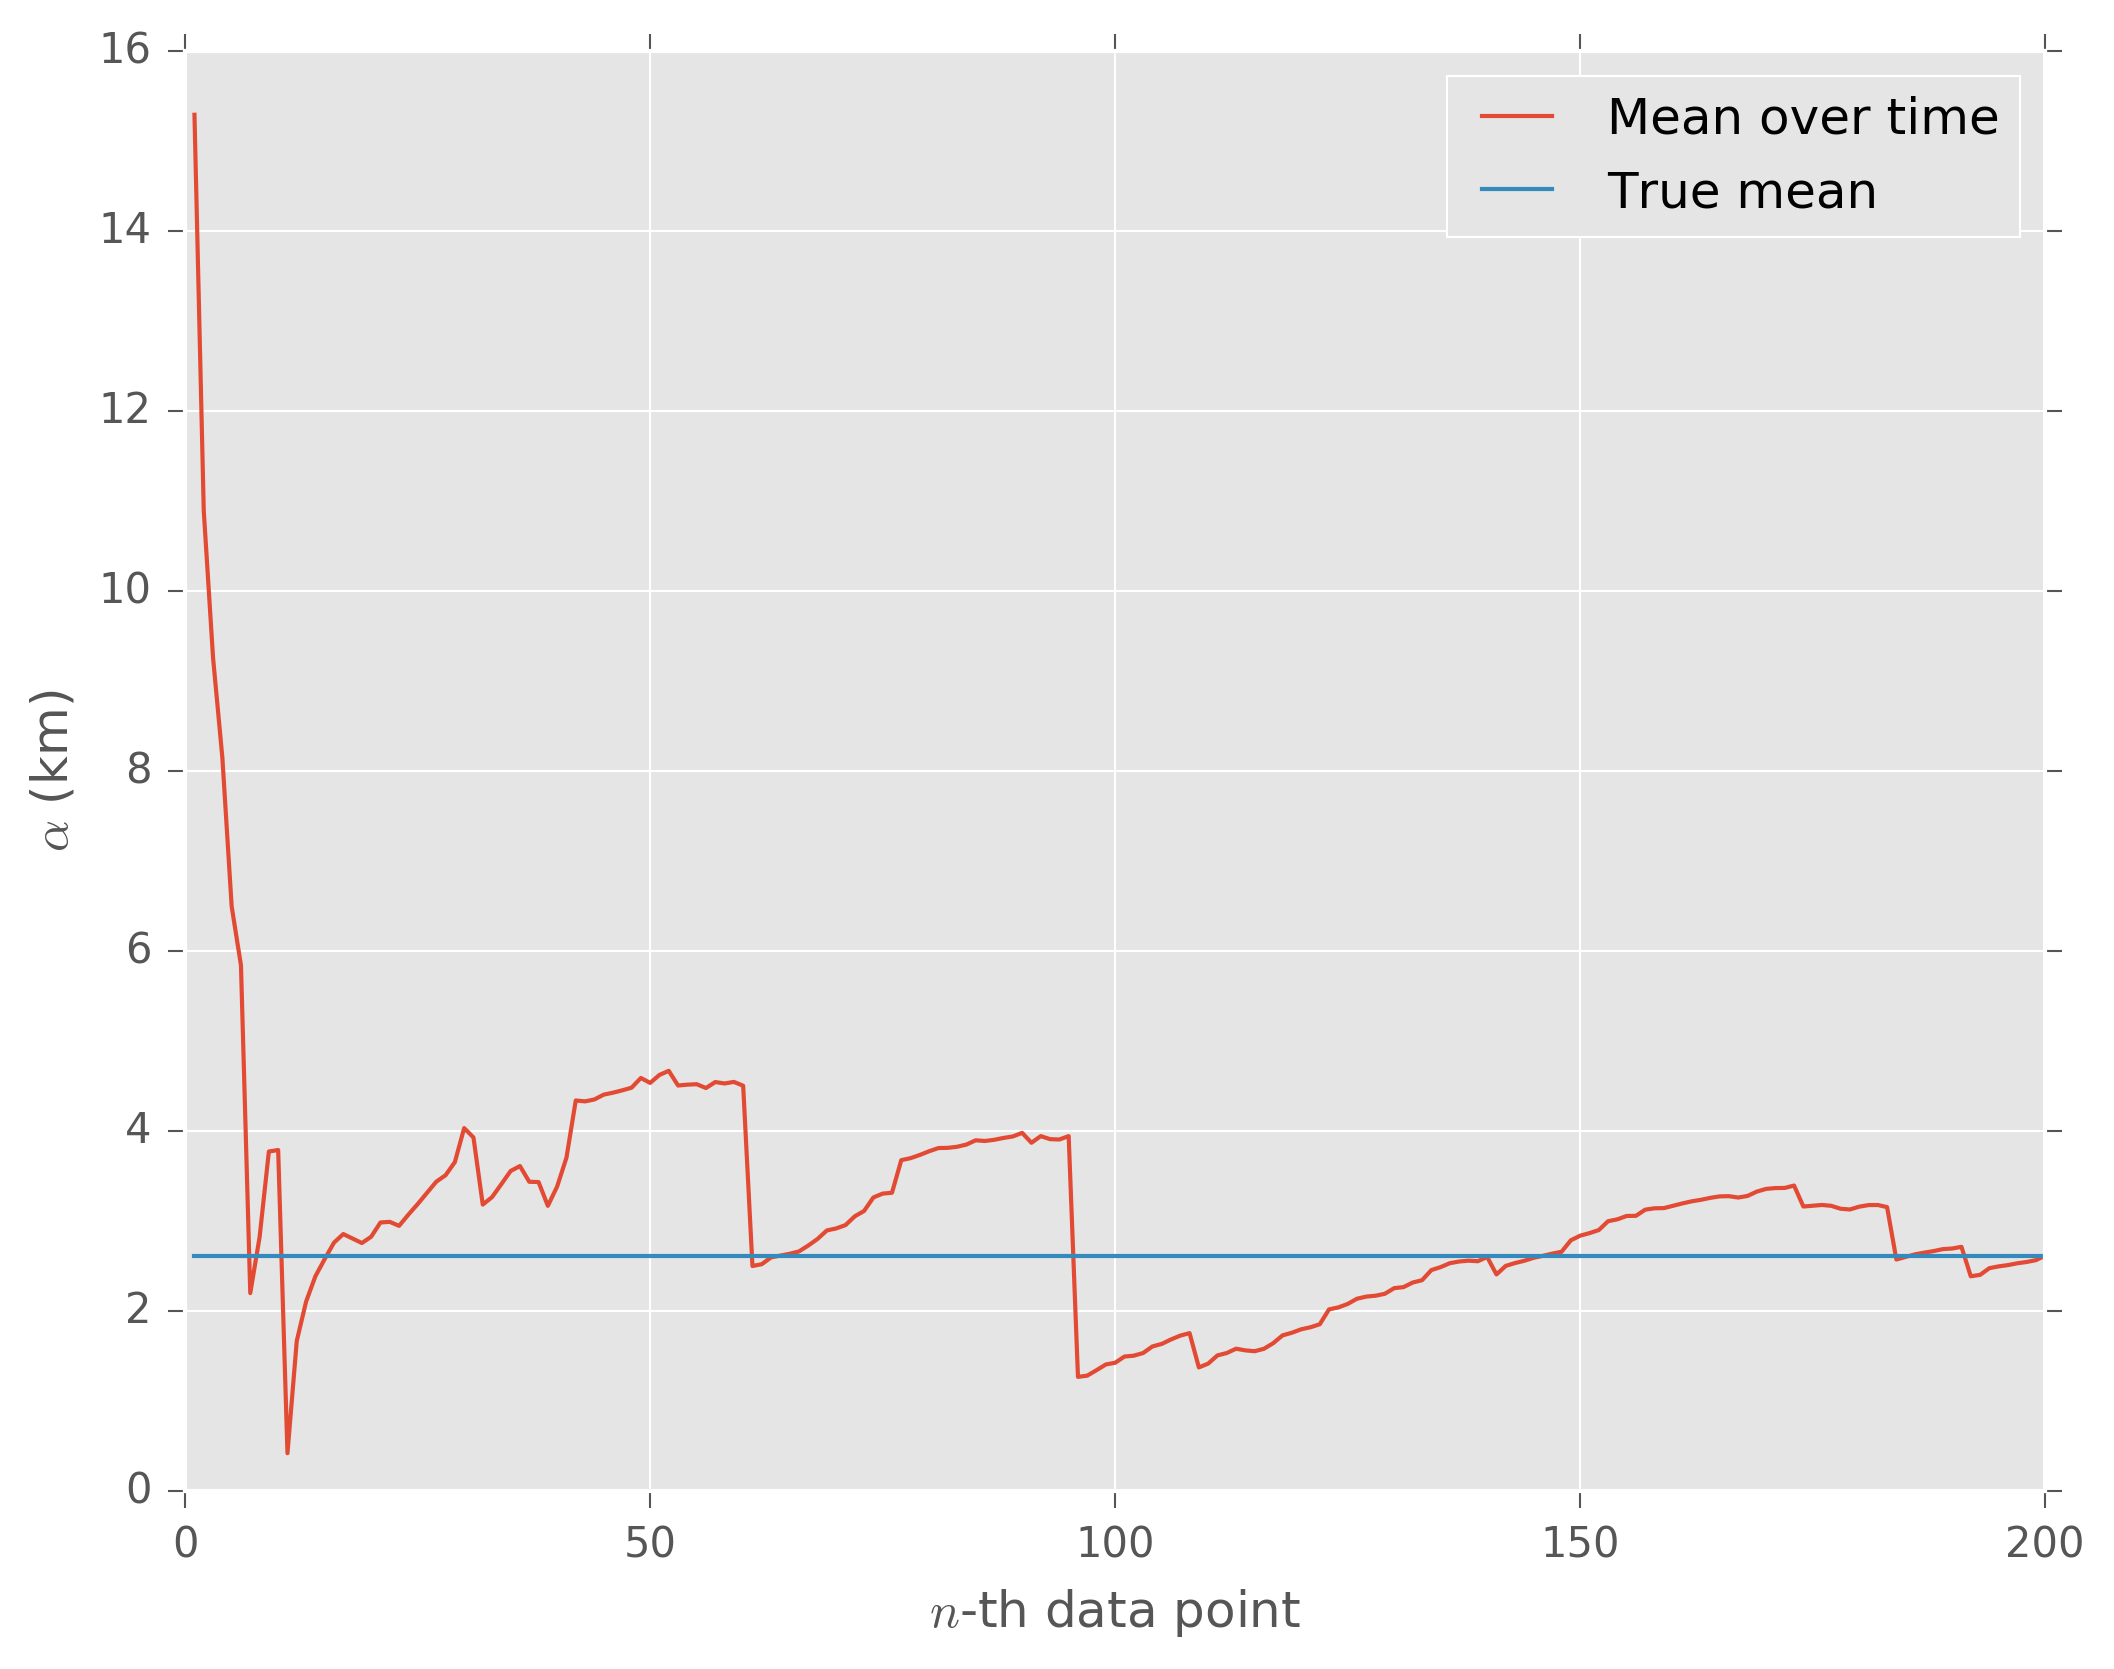
\includegraphics[width=.6\textwidth]{images/mean_x.png}
\caption{Mean of $x$ as a function of the number of datapoints (Ex 2.2.3)}
\end{figure}
The mean of the data is 2.61. This is not close to the true position of the lighthouse ($\alpha = 6.03$). The mean over time is at the beginning also quite far off, but starts getting closer towards the end. I reckon 150 points is a good lower bound for the necessary number of data points.
\end{enumerate}
\subsection*{Part 3 -- Find the lighthouse}
\begin{enumerate}
\item 
\begin{align*}
p(\mathcal{D} | \alpha, \beta) &= \prod_{k=1}^N p(x_k | \alpha, \beta) \\
\ln p(\mathcal{D} | \alpha, \beta) &= \ln\prod_{k=1}^N p(x_k | \alpha, \beta) \\
&= \sum_{k=1}^N\ln p(x_k | \alpha, \beta) \\
&= \sum_{k=1}^N\ln\frac{\beta}{\pi[\beta^2+(x_k - \alpha)^2]} \\
&= N\ln\frac{\beta}{\pi} - \sum_{k=1}^N \ln[\beta^2+(x_k - \alpha)^2]
\end{align*}
This is similar to Exericise 2.1.3
\item 
\begin{figure}[H]
\centering
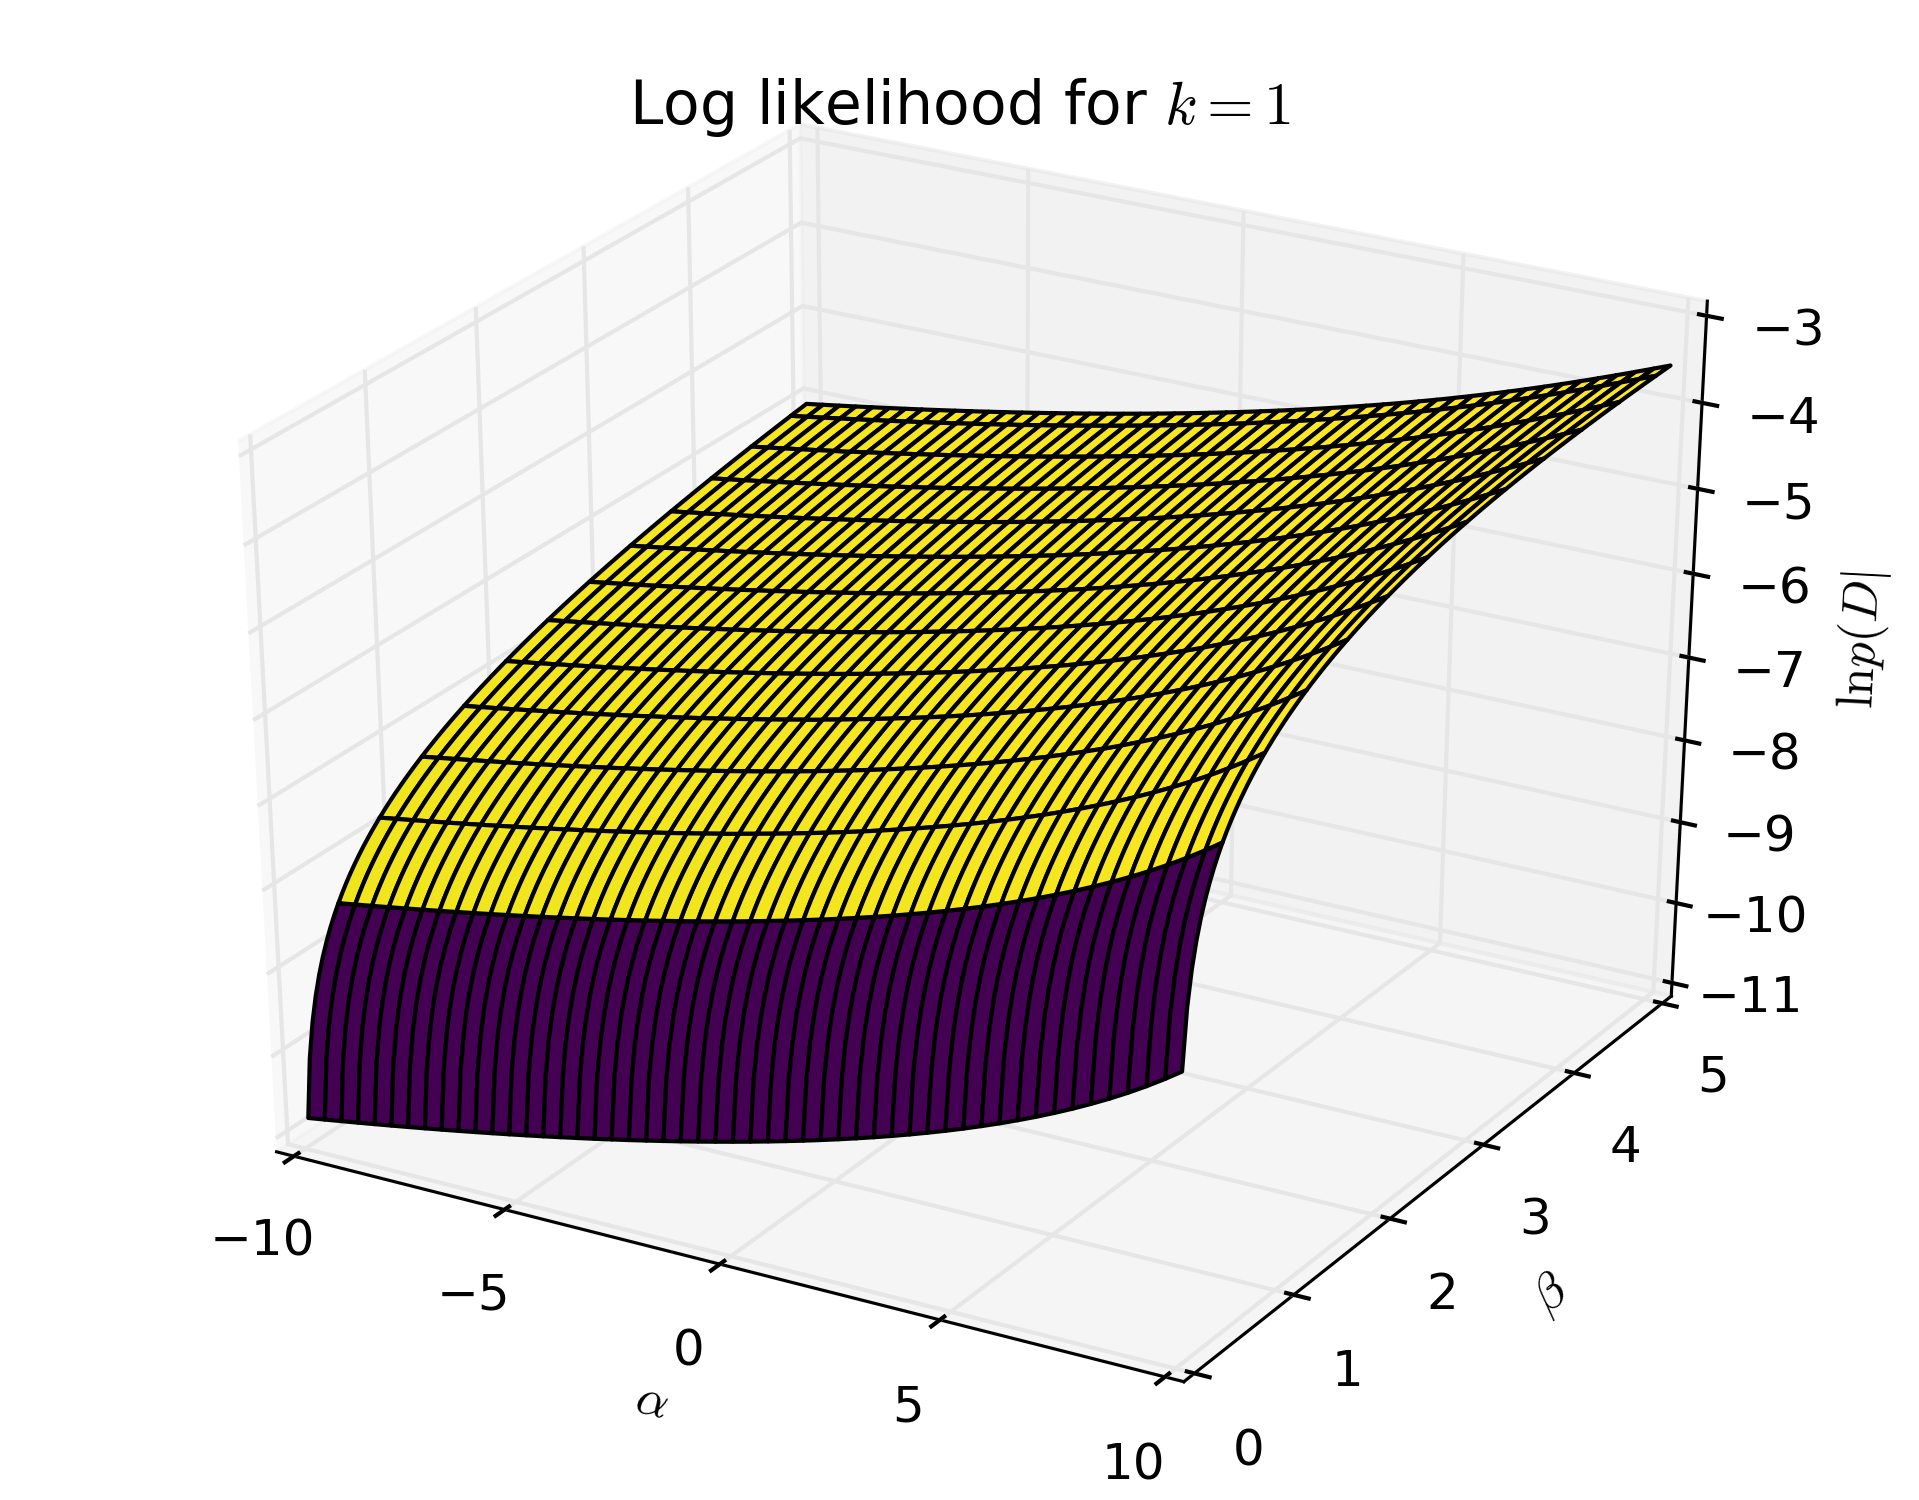
\includegraphics[width=.45\textwidth]{images/logl_1.png}
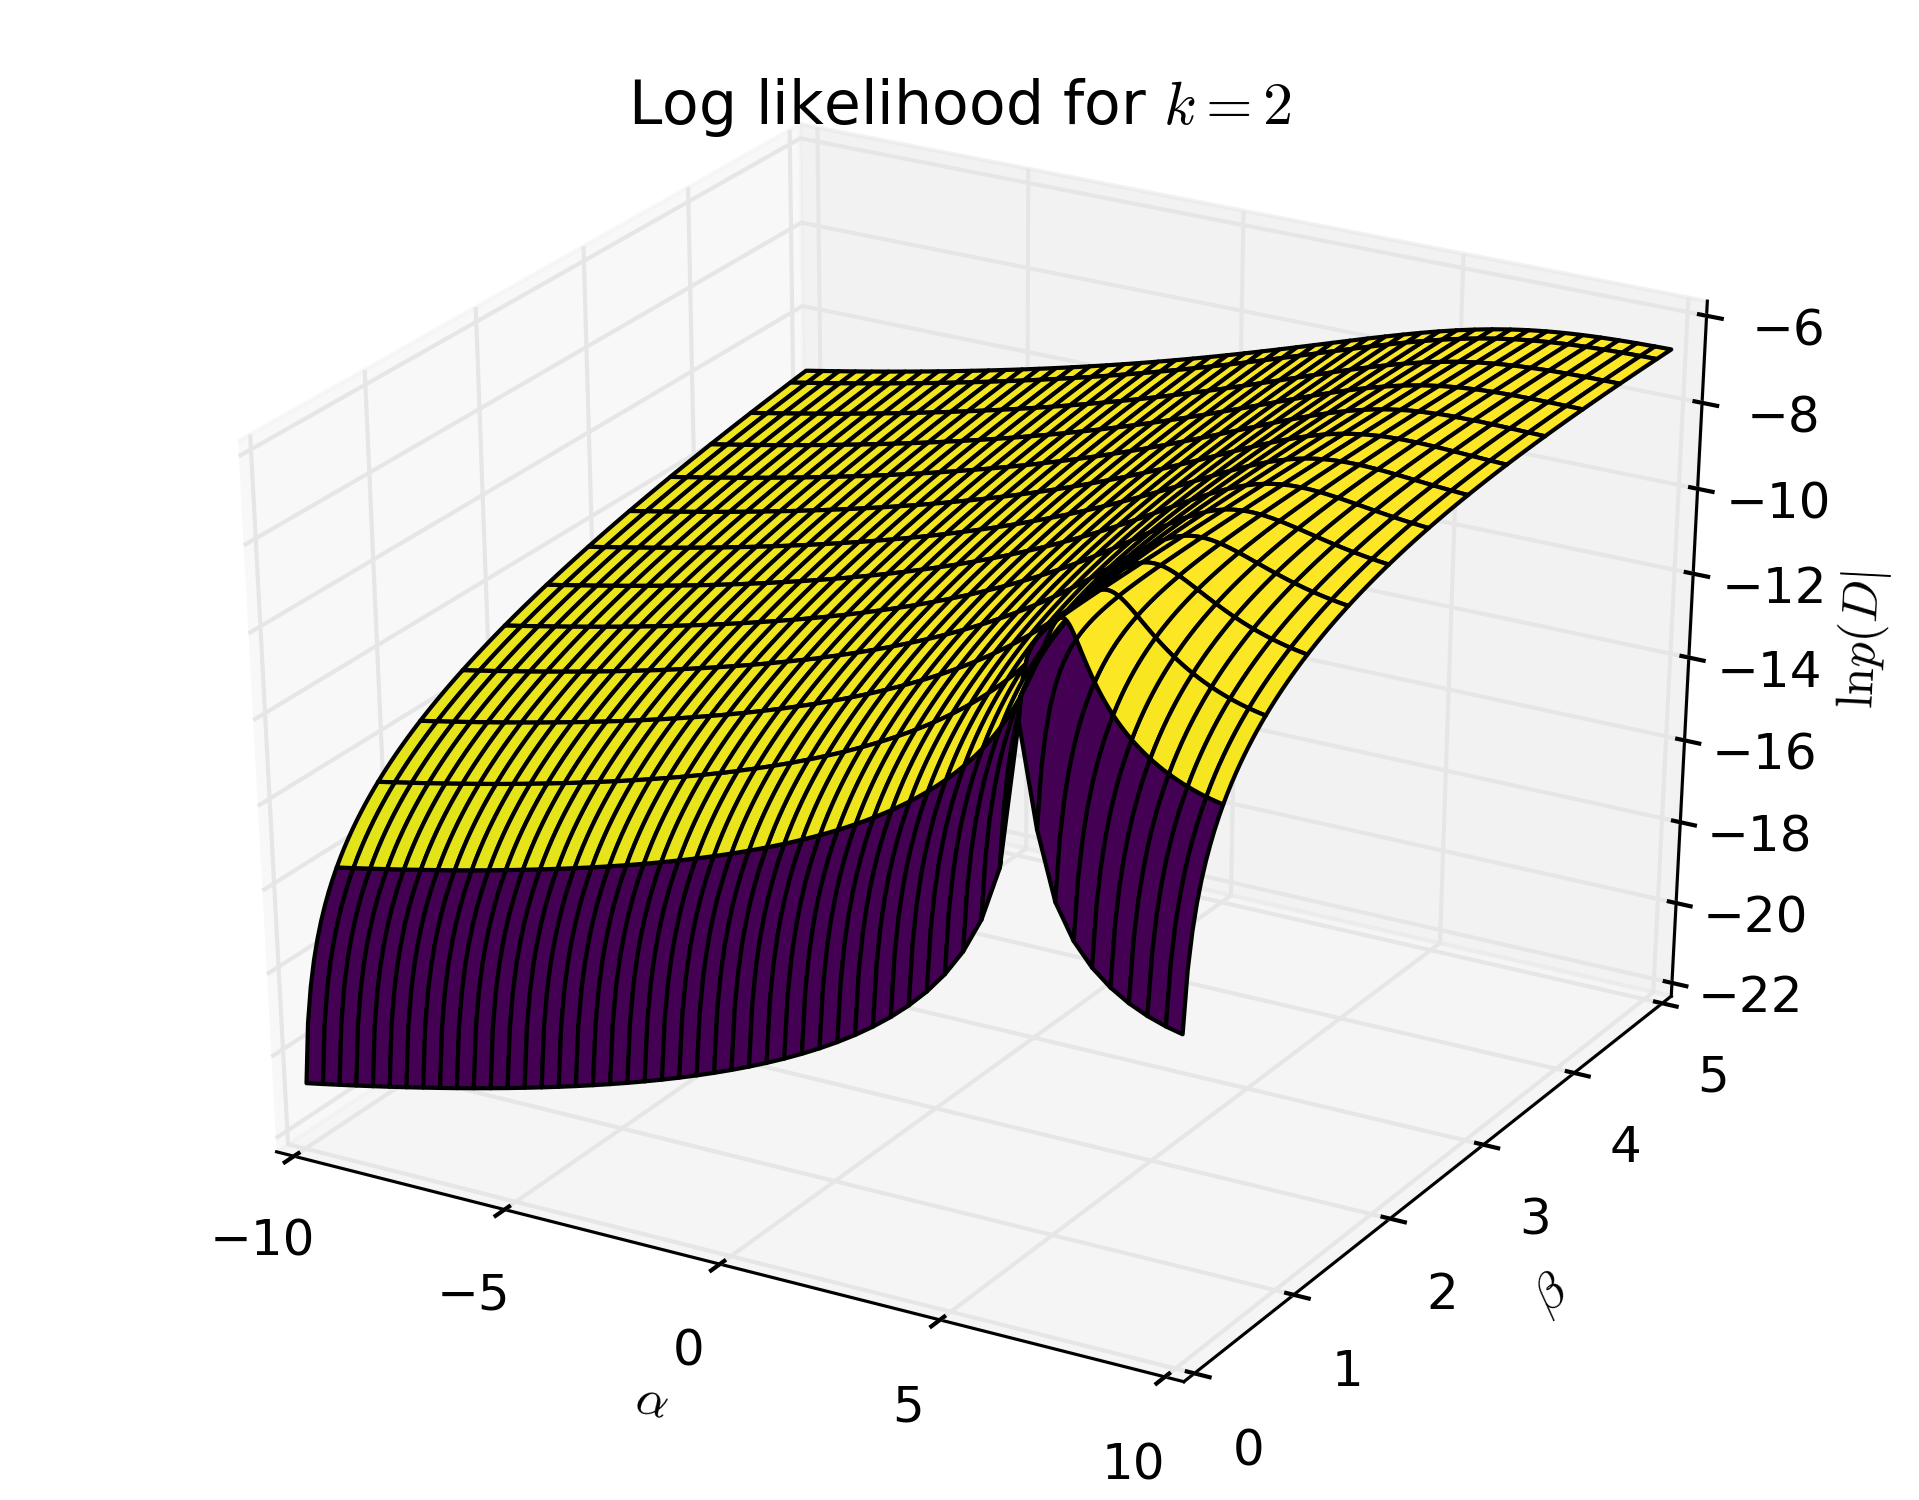
\includegraphics[width=.45\textwidth]{images/logl_2.png}
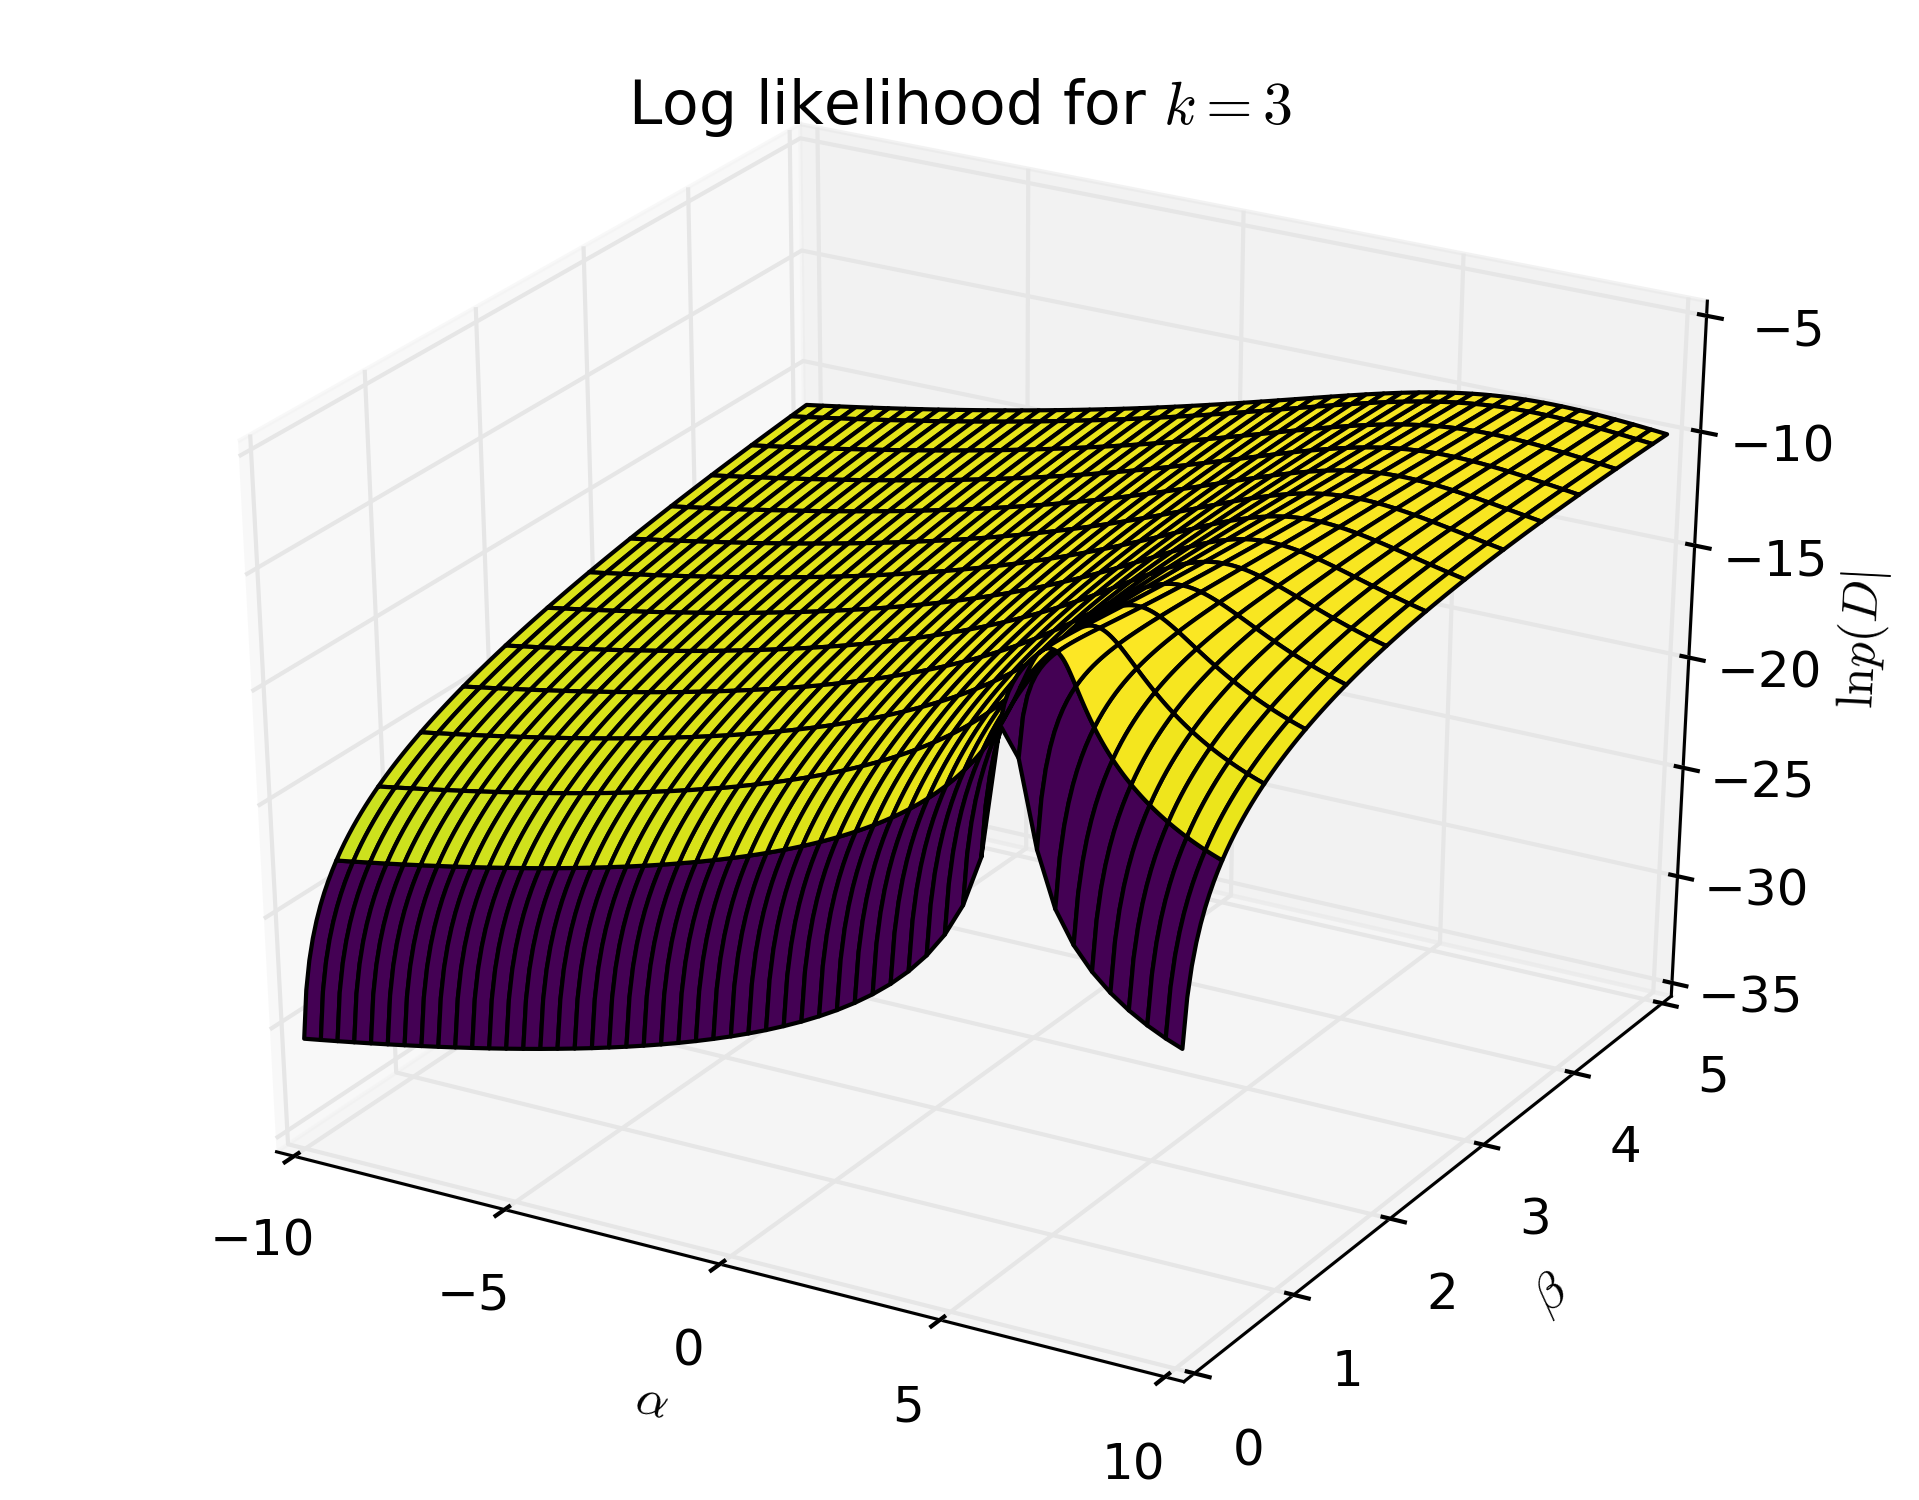
\includegraphics[width=.45\textwidth]{images/logl_3.png}
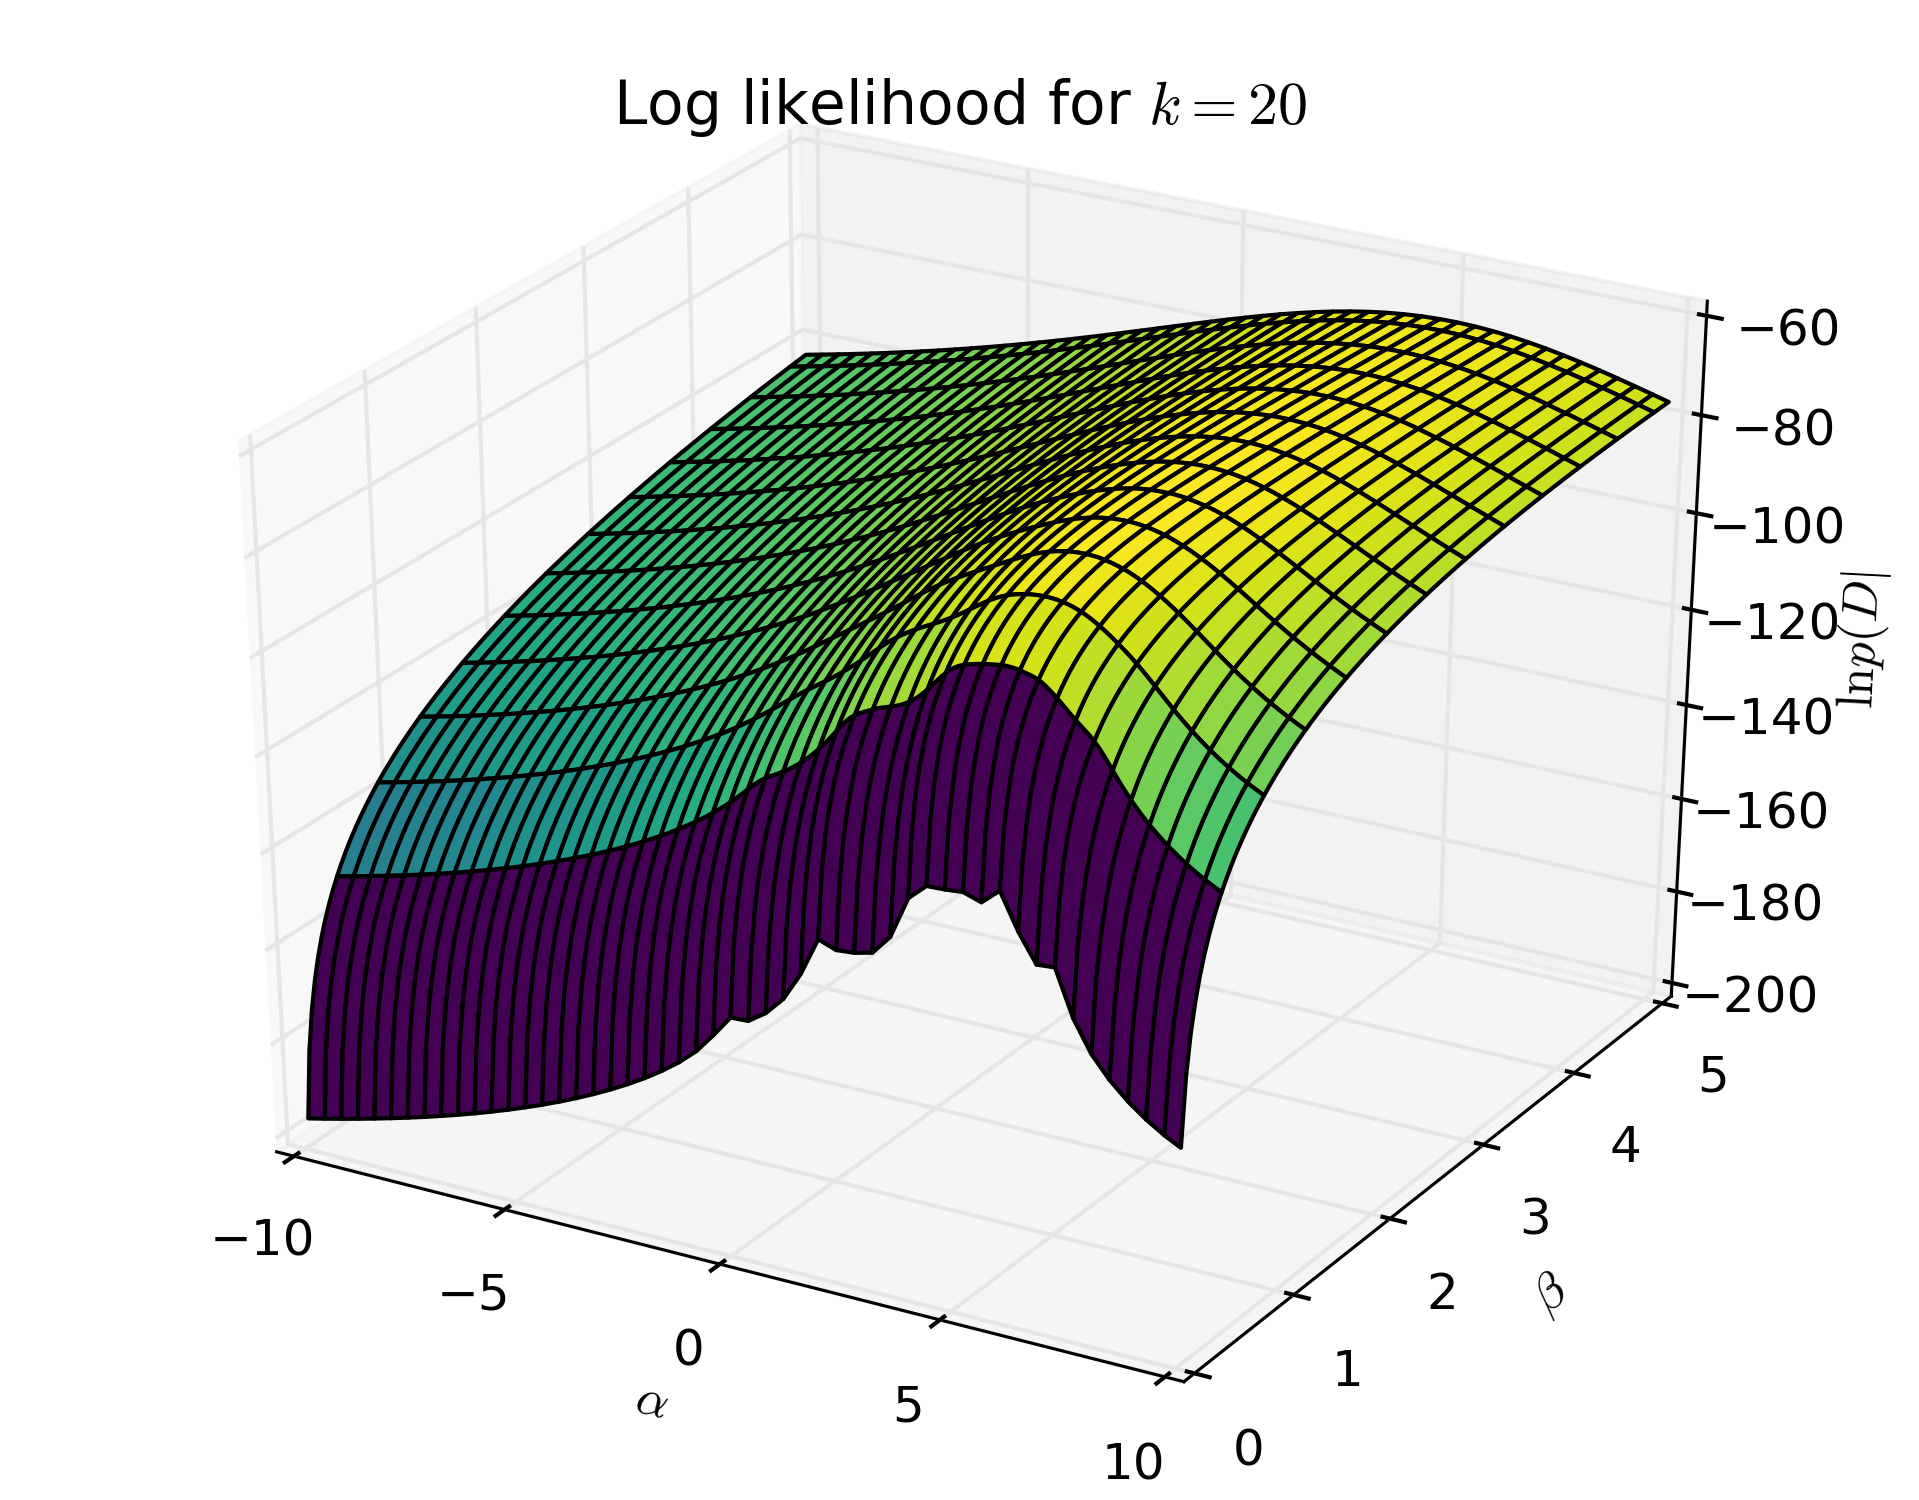
\includegraphics[width=.45\textwidth]{images/logl_20.png}
\caption{Log likelihood for $\alpha$ and $\beta$ for different numbers of datapoints (Ex 2.3.2)}
\end{figure}
\begin{python}
ks = [1, 2, 3, 20]
alphas, betas = np.mgrid[-10:10:0.04, 0:5:0.04]
# alphas, betas = np.meshgrid(np.linspace(-10, 10, num=500), np.linspace(0, 5, num=250))
for k in ks:
    x = locations[:k]
    # We only have to calculate the constant once
    likelihood = k * np.log(betas/np.pi)
    for loc in x:
        likelihood -= np.log(betas**2 + (loc - alphas)**2)
        
    fig = plt.figure()
    ax = fig.gca(projection='3d')
    ax.plot_surface(alphas, betas, likelihood, cmap=plt.cm.viridis)
    # And some more plot formatting code
\end{python}
With few datapoints, it is not very likely that de lighthouse is close to the coast. This is because a lighthouse really close to the coast would result in few data points close to that position. As more points come in, this does become more likely. We also see that the likelihood starts increasing around $a_t$ as more points are considered. 
\par The log-likelihood does not suffer from numerical precision errors after multiplication of a lot of small numbers. The expression may also be easier to compute. However, it is not a probability distrubition and can thus not directly be compared with other distributions.
\item 
\begin{python}
from scipy.optimize import fmin

def log_likelihood(params, locations):
    """
    This function will be minimized.
    This is why it returns -likelihood
    """
    alpha, beta = params
    likelihood = len(locations) * np.log(beta/np.pi)
    for loc in locations:
        likelihood -= np.log(beta**2 + (loc - alpha)**2)
    return -likelihood
    
def plot_maximize_logl(data):
    alphas, betas = [], []
    x = np.arange(len(data))
    for k in x:
        [alpha, beta] = fmin(log_likelihood, (0, 1), args=(data[:k],))
        alphas.append(alpha)
        betas.append(beta)
    
    return alphas, betas
\end{python}
\begin{figure}[H]
\centering
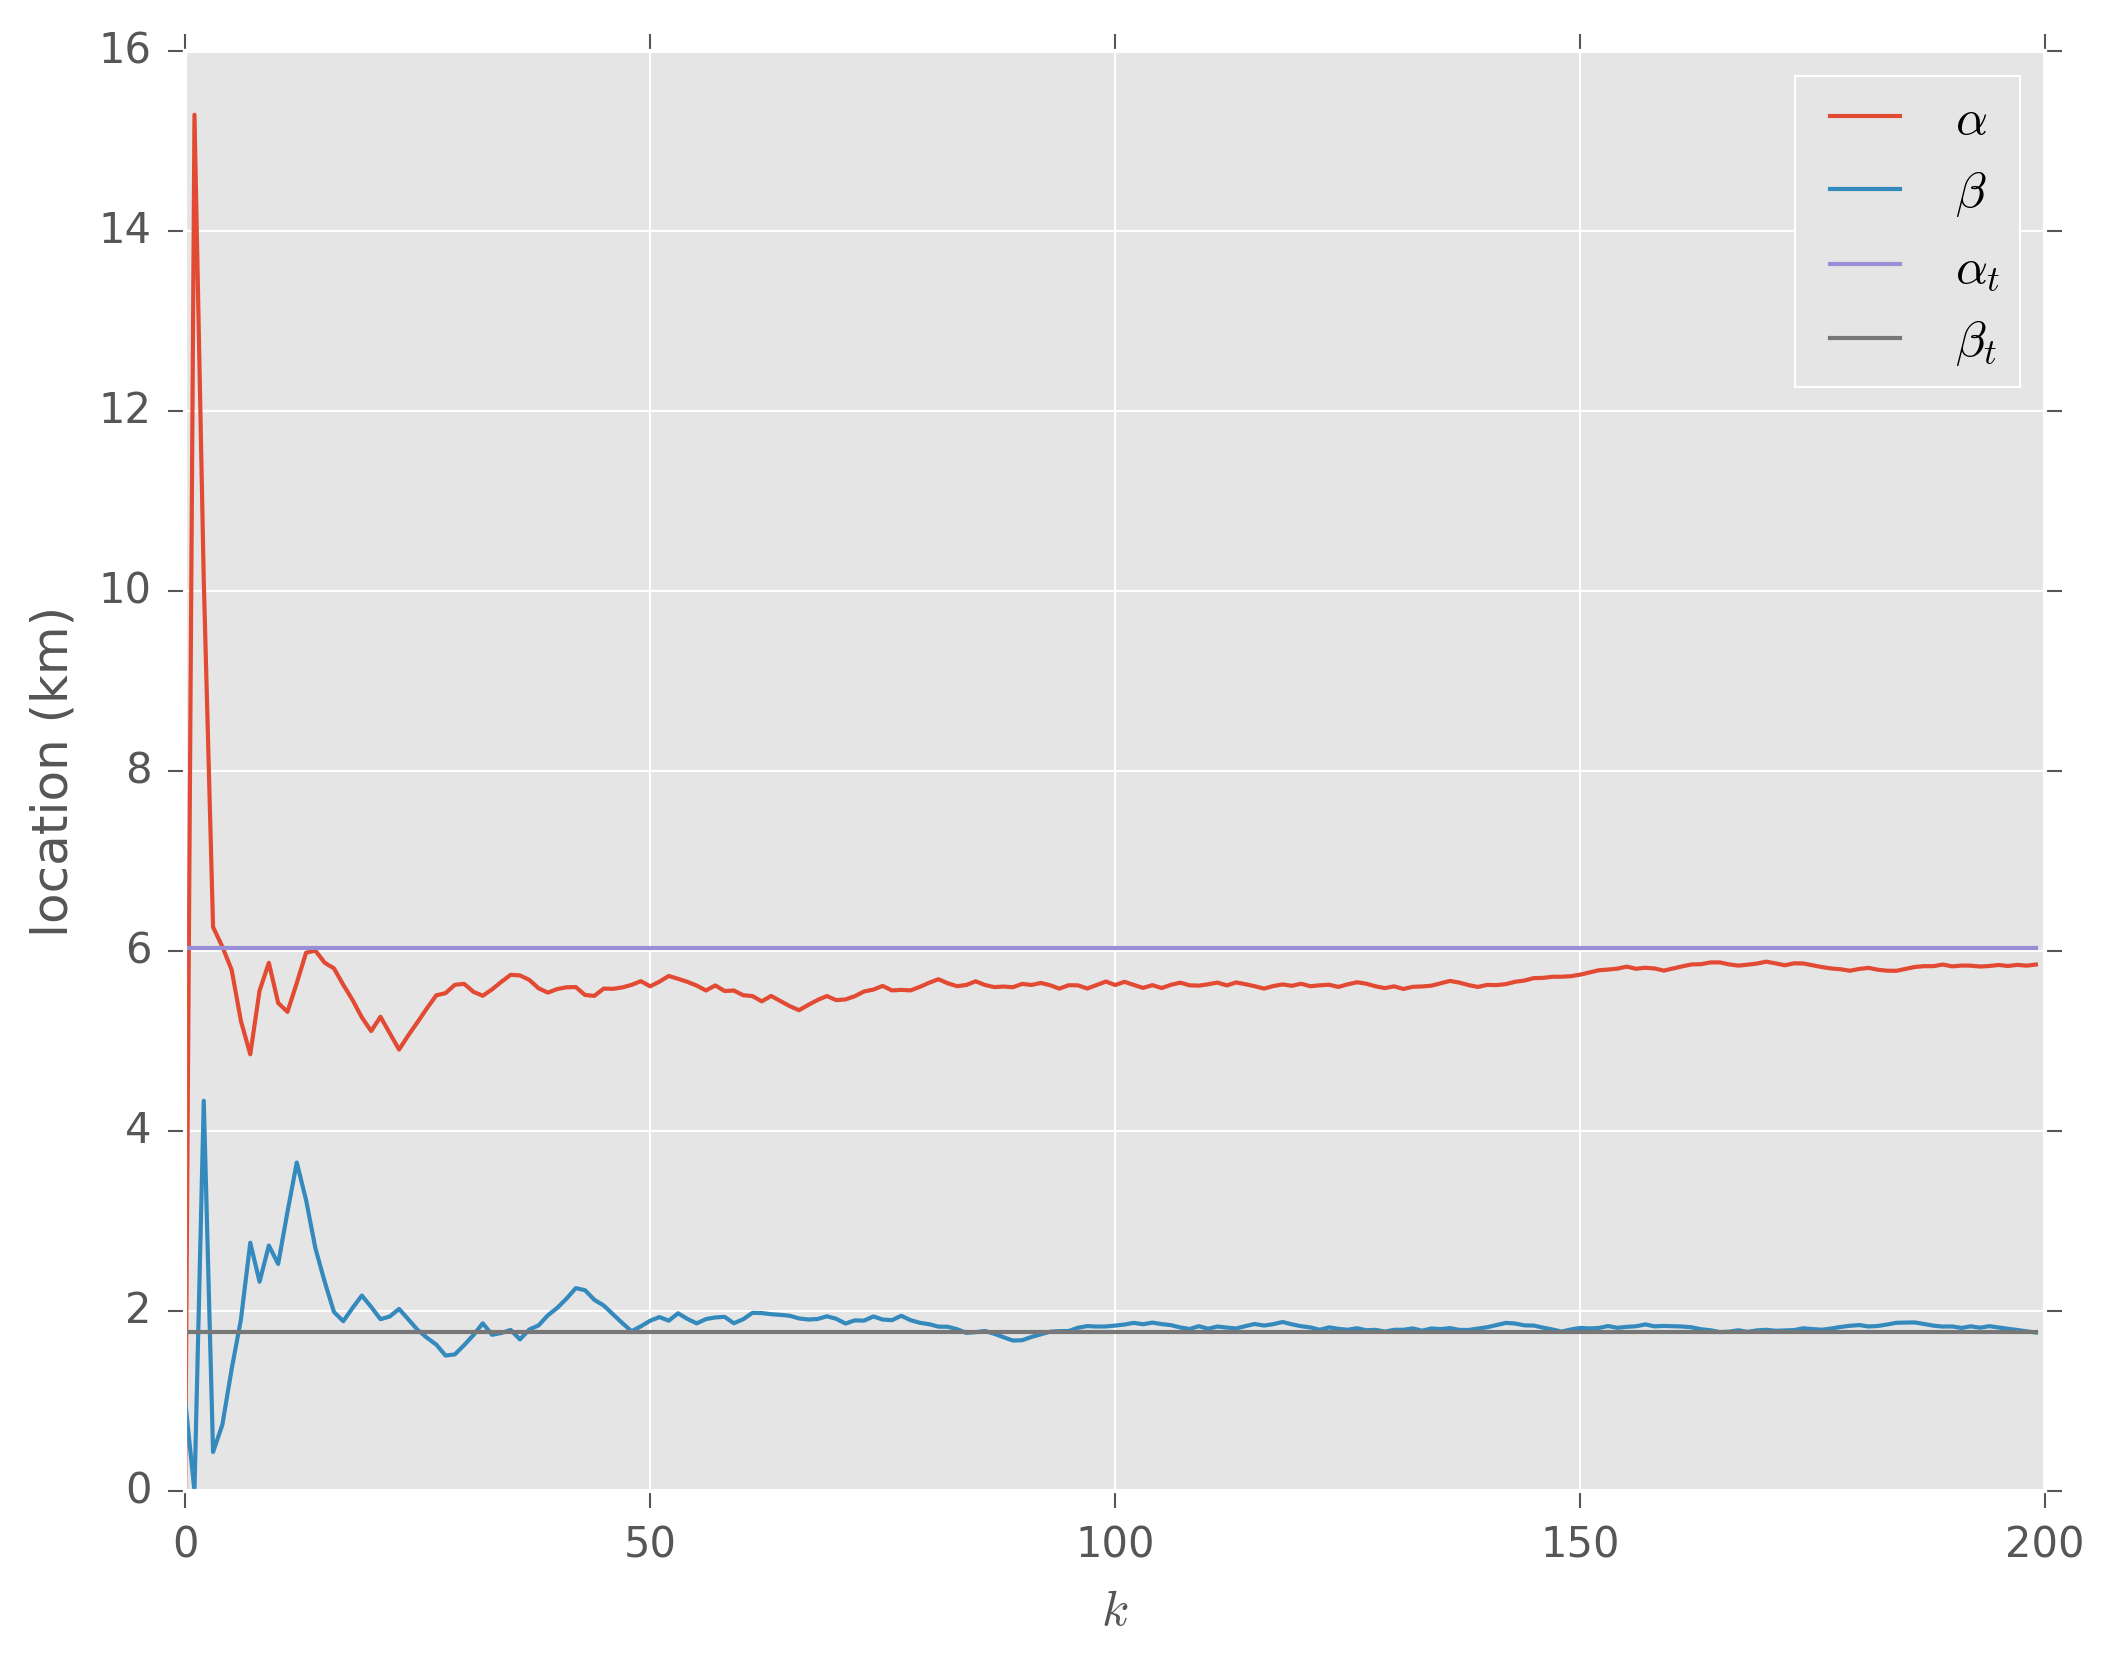
\includegraphics[width=.6\textwidth]{images/min_logl.png}
\caption{The maximum likelihood estimate of $\alpha$ and $\beta$ as a function of the number of data points. (Ex 2.4.3)}
\end{figure}
When considering all 200 data points, the point $\alpha = 5.85$ and $\beta = 1.76$ yield the highest likelihood. This is close to the real position ($\alpha_t = 6.03$ and $\beta_t=1.76$). The estimates converge to their true values relatively fast (a lot faster than I estimated in 2.2.3)
\end{enumerate}
\end{document}